\chapter{楽曲制作}
\section{NoteSequenceについて}
NoteSequenceとはMIDIデータから作成されるプロトコルバッファである.
プロトコルバッファとはGoogleが2008年にオープンソース化したバイナリベースのデータフォーマットである.
既存の技術としてはXMLやJSONなどのテキストベースのデータフォーマットがあるが,プロトコルバッファはバイナリフォーマットであるので,アプリケーション間でデータ構造の送受信をする際に少ないデータ量ですむという特徴がある.
スキーマ言語はなぜ重要なのか、そういう時代になったからだ.
我々が単一RDBに接続する単一のWebアプリだけを書いていられる時代はとうの昔に終わった。データはあちこちのいろんなストレージ技術で保存されているかもしないし、バックエンドも単一サービスではなくて分割されているかもしれないし、クライアントはweb版, iOS版, Android版があってひょっとしたらそれぞれ別の言語で実装されており、外部開発者向けにAPIも公開しなければならない。
だから、そこら中でデータをシリアライズするしデシリアライズするし、通信の両端で解釈に矛盾が無いようにすり合わせる必要がある。でも、すりあわせの目的でいちいち人間と自然言語で会話するのは苦痛なので、私たちは機械処理可能なコードで語りたい。だから、どういうデータがやってくるのかきちんと宣言的DSLで定義しておきたい。そこでスキーマ言語だ。
JSON Schemaが広がりつつあるのもたぶんそういう理由だし、そもそもProtobuf自体もGoogleが社内で同じ問題にぶち当たって発明されたんだったような気がする。
自分の管轄領域内に閉じたデータ構造であれば、スキーマとか型宣言とか細かい縛りなしで軽量に進めるのもありだ。しかし、他人の領域との界面はしっかり定義しておいた方が良い。スキーマ定義という税金を支払わないとその分のツケはどこかで回ってきて、1時間掛かるE2Eテストがこけるとか、週次変更レビュー合同会議の発足とか、そういうやつで支払うことになる。
スキーマ定義さえあれば、webクライアント開発用の, バックエンド開発用の, アプリ開発用の言語に向けて対応するデータ構造定義を自動生成して、矛盾なくすべてをメンテナンスできる。
通信の両端でスキーマさえ合致していれば、シリアライゼーション形式を合わせるのはむしろ間違えづらい。だから、JSONでもProtobufのデフォルトのそれでも、MessagePackでもXMLでも好きにすれば良い。ちなみに、Protobufで定義したデータ構造はProtobuf標準形式の他にJSONにもきちんとシリアライズできる。
\section{NoteSequenceの作成}
NoteSequenceの作成は図のコマンドで作成できる.
\begin{figure}[!ht]
    \begin{screen}
    \begin{center}
        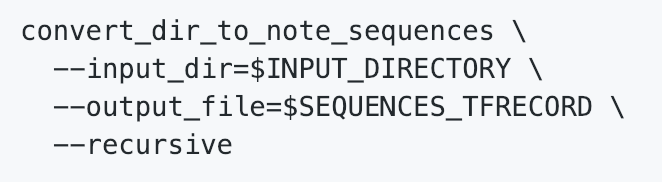
\includegraphics[scale=0.7, clip]{./img/Notesequence_make.png}
        \caption{NoteSequenceの作成}
        \label{fig:NoteSequenceの作成}
    \end{center}
    \end{screen}
\end{figure}\\
--input\_dirで学習させるMIDIデータのディレクトリの絶対パスを指定し,--output\_fileでNotesequenceの出力先のディレクトリを指定する.\\
次に作成したNoteSequenceのデータセットを学習用と評価用に分割するために,下記のコマンドを実行する.
\begin{figure}[!ht]
    \begin{screen}
    \begin{center}
        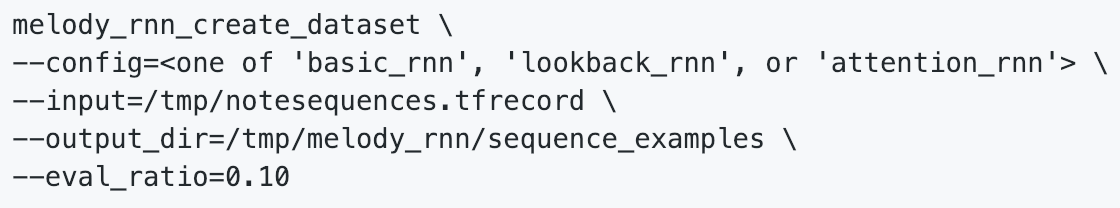
\includegraphics[scale=0.7, clip]{./img/Notesequence_split.png}
        \caption{NoteSequenceを学習用と評価表に分割}
        \label{fig:NoteSequenceを学習用と評価表に分割}
    \end{center}
    \end{screen}
\end{figure}\\
--configで使用するRNNを指定する.--input\_dirでNoteSequenceの絶対パスを指定し,--output\_fileで分割したNotesequenceの出力先のディレクトリを指定する.
--eval\_ratioでNotesequenceのデータを何パーセント学習用に用いるかを指定する.コマンドの場合は10\%が学習用のデータになる.
\subsection{学習の開始}
作成したNoteSequenceから学習モデルを作成するために下記のコマンドを実行する.
\begin{figure}[!ht]
    \begin{screen}
    \begin{center}
        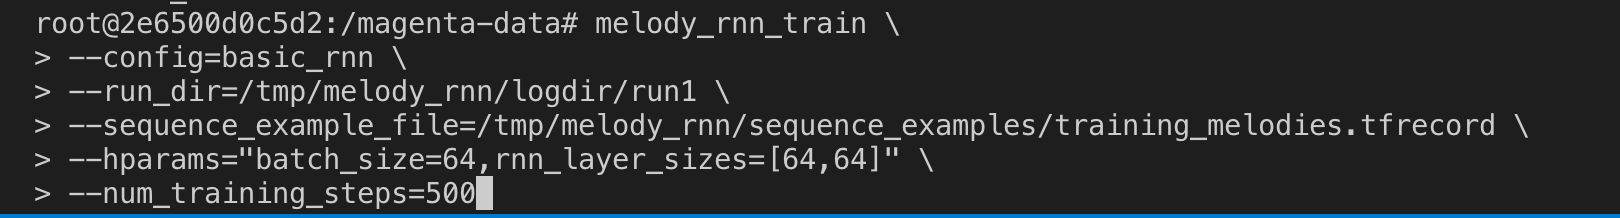
\includegraphics[scale=0.5, clip]{./img/Rnn_train.png}
        \caption{BasicRNNを使用した学習の開始}
        \label{fig:BasicRNNを使用した学習の開始}
    \end{center}
    \end{screen}
\end{figure}\\
--configで学習に使用する学習モデルを指定,--rundirで学習モデルの出力先のディレクトリを指定し,--sequence\_examplefileで学習のために用意したNotesequenceを指定する.
--hparamsでメモリの使用量を指定し,--rnn\_layer\_sizeで中間層のノード数を指定し,--num\_trainingstepsで学習回数を設定する.\\
\subsection{音楽データの作成}
下図のコマンドで学習モデルに入力する 音調をMIDIの形式で 指定し音楽データを作成する.
\begin{figure}[!ht]
    \begin{screen}
    \begin{center}
        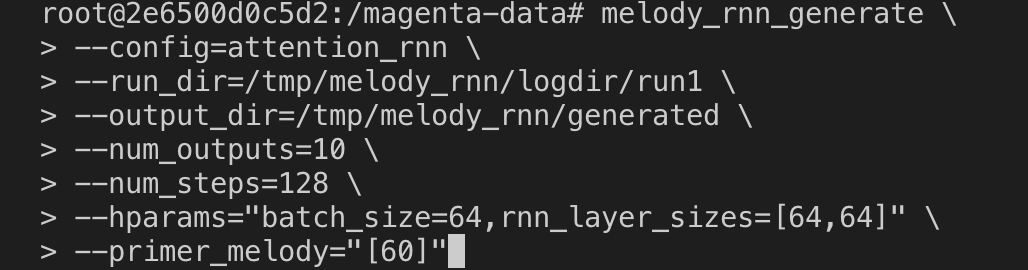
\includegraphics[scale=0.7, clip]{./img/MIDI_make.png}
        \caption{学習モデルを使用し,10曲を作成}
        \label{fig:学習モデルを使用し,10曲を作成}
    \end{center}
    \end{screen}
\end{figure}